\documentclass[10pt]{article}
\usepackage{amssymb,amsmath,times,url,graphicx,amsthm,alltt}
%\usepackage[pdftex,urlcolor=blue,pdfpagemode=none,pdfstartview=FitH]{hyperref}
\usepackage{my_packages}
\usepackage{tikz_packages}
%% url smaller font.
\makeatletter
\def\url@leostyle{%
  \@ifundefined{selectfont}{\def\UrlFont{\sf}}{\def\UrlFont{\small\ttfamily}}}
\makeatother
\urlstyle{leo}

%\usepackage[all,import]{xy}

\renewcommand{\baselinestretch}{1.2}
\date{}

\renewcommand{\thesubsection}{\arabic{subsection}. }
\renewcommand{\thesubsubsection}{\arabic{subsection}.\arabic{subsubsection} }

\theoremstyle{definition}
\newtheorem{prob}{Problem}[section]
%\renewcommand{\theprob}{\arabic{section}.\arabic{prob}}
\renewcommand{\theprob}{\arabic{prob}}

\newenvironment{subprob}%
{\renewcommand{\theenumi}{\alph{enumi}}\renewcommand{\labelenumi}{(\theenumi)}\begin{enumerate}}%
{\end{enumerate}}%

\newenvironment{matlab}
{\begin{alltt}\small\renewcommand{\baselinestretch}{1.2}\selectfont}%
{\end{alltt}}


\begin{document}



\setcounter{page}{1}
\pagestyle{plain}
\section*{MAE3145: Homework 4}
\vspace*{-0.4cm}
\noindent{Due date: \SI{2458038.1979166665}{\julianday} }%\\%\vspace*{0.5cm}

\begin{prob}
    Halley's comet last passed through perihelion on Feb 9, 1986.
    The orbit is described with an eccentricity of \( e = 0.9671429\) and a semi-major axis of \( a = 17.834144 \si{\astronomicalunit} \).
    In 1986, the European Space Agency spacecraft Giotto encountered and photographed teh nucleus of the comet as it approached the Sun.
    Data from Giotto's camera was used to generate the enhanced image shown in~\cref{fig:halley}.
    \begin{figure}[htbp]
        \centering
        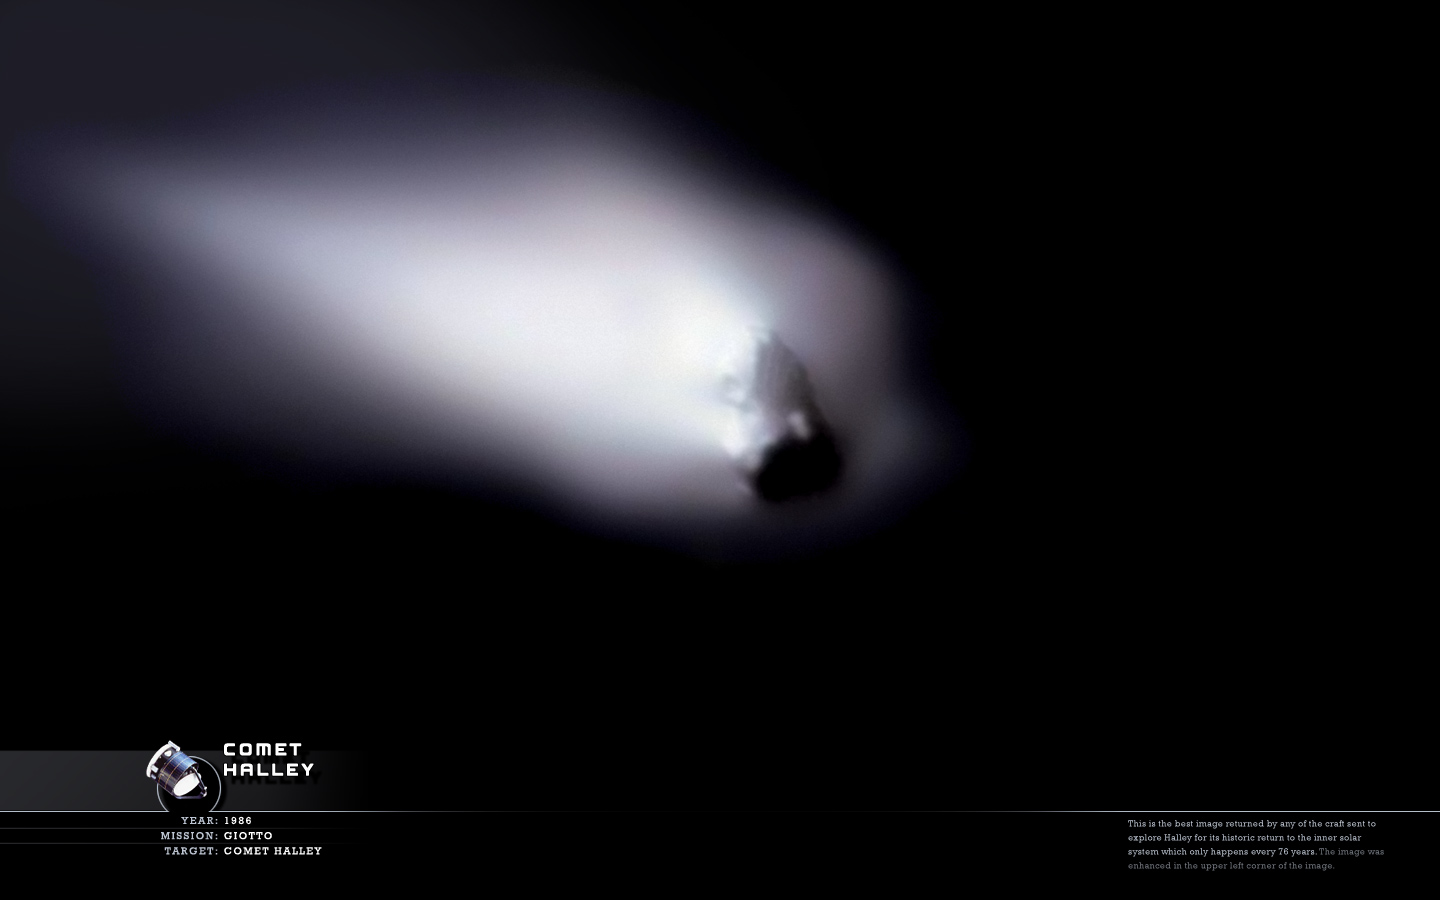
\includegraphics[width=0.75\textwidth, keepaspectratio]{figures/halley.jpg}
        \caption{Halley's Comet as seen by Giotto\label{fig:halley}}
    \end{figure}
    The potatoe shaped nucleus measures roughly \SI{15}{\kilo\meter} across and is composed primarily of water and carbon dioxide ices.

    \begin{subprob}
    \item On this date, determine the following additional orbital characteristics associated with Halley's orbit (assume a conic model):
        \begin{align*}
            r, \quad v, \quad \nu, \quad \gamma, \quad \mathcal{E}, \quad h, \quad \mathsf{P}, \quad r_a, \quad r_p, \quad E
        \end{align*}
        Ensure that you list all distances in astronomical units.
    \end{subprob}

    You can check the path of 1P/Halley at the JPL Small-Body Data Browser by going to the following \href{https://ssd.jpl.nasa.gov/sbdb.cgi?ID=c00001_0}{link}.
        Observers on Earth can pick up the comet when its true anomaly is approximately \SI{100}{\degree} prior perihelion.
    \begin{subprob}
    \item Determine the same quantities shown in part (a) above, but at the time when the observers expect to pick up the next return.
    \item Determine the time required to go from the last perihelion passage to the location where Earth observers can again pick up the return of Halley's Comet.
        What is the approximate date?
        How old will you be?
    \item How many days until the comet passes through perihelion?
\end{prob}

\begin{prob}
    A satellite is in orbit about the Earth. 
    Assume that it is reasonable to model the behavior in terms of the relative two-body problem (Earth and Satellite).

\end{prob}
\end{document}


